\documentclass{beamer}
\usepackage{graphicx}
\usepackage{tikz}
\usetikzlibrary{shapes,arrows}
\usepackage{tikz}
\usetheme{default}
%\usecolortheme{seahorse}
\usepackage{default}

  \setbeamertemplate{footline}[page number]
\setbeamertemplate{navigation symbols}{}
\setbeamertemplate{frametitle}[default][center]
\setbeamerfont{frametitle}{shape=\scshape}

\usepackage{color}

{\title{\textsc{Intertemporal Lecture}}
\author{Trevor S. Gallen}
\date{}



\begin{document}


\begin{frame}
\titlepage
\end{frame}

\begin{frame}
\frametitle[alignment=center]{Intertemporal Economics}
\begin{itemize}
\item So far our labor/consumption model was ``static" (no multiple periods)
\bigskip
\item But so much of human behavior is lifecycle/dynamic
\bigskip
\item We'll give a crash course on dynamic econ
\end{itemize}
\end{frame}

\begin{frame}
\frametitle[alignment=center]{Intertemporal Economics}
\begin{itemize}
\item So far our labor/consumption model was ``static" (no multiple periods)
\bigskip
\item But so much of human behavior is lifecycle/dynamic
\bigskip
\item We'll give a crash course on dynamic econ
\bigskip
\item We'll do even less theory because it's far outside scope of course
\end{itemize}
\end{frame}


\begin{frame}
\frametitle[alignment=center]{Intertemporal Economics}
\begin{itemize}
\item We'll think just about consumption $u(c_1,c_2)$
\bigskip
\item It's possible happiness between the two is connected (``habit formation") but mostly we model it as:
$$u(c_1,c_2)=u(c_1)+\beta u(c_2)$$
\item Where $\beta$ is some ``impatience" factor (``discount rate")
\bigskip
\item Budget constraint(s) (endowment $I$) becomes:
$$I_1=c_1+s_{1\rightarrow 2}$$
$$I_2+(1+r)s_{1\rightarrow 2}=c_2$$
\item Combining the two by cancelling savings to get the ``net present value" budget constraint:
$$I_1+\frac{I_2}{1+r}=c_1+\frac{c_2}{1+r}$$
\item What does BC look like?
\end{itemize}
\end{frame}

\begin{frame}
\frametitle[alignment=center]{Intertemporal Economics}
\begin{figure}
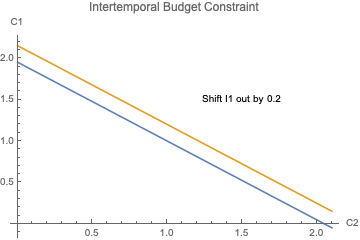
\includegraphics[scale=0.85]{ITBC1.png}\end{figure}
\end{frame}

\begin{frame}
\frametitle[alignment=center]{Intertemporal Economics}
\begin{figure}
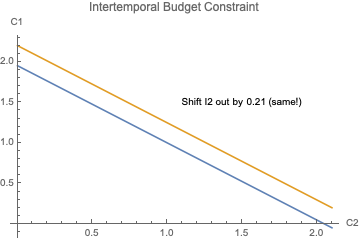
\includegraphics[scale=0.85]{ITBC2.png}\end{figure}
\end{frame}

\begin{frame}
\frametitle[alignment=center]{Testable Predictions}
\begin{itemize}
\item Important implication and predictions (science!)
\smallskip
\item Let's say Trevor earned \$100 today and next year (then died).  How much should he consume in each period?
\smallskip
\item<2->  Prediction:  probably about \$100 in each year (why?)
\smallskip
\item<3->  He likes to smooth consumption!
\smallskip
\item What if you give Trevor \$50 extra today?  How much more consume today vs tomorrow?
\smallskip
\item If he likes to smooth, \$125.61 today and \$125.61 tomorrow 
$$\underbrace{126.61}_{\text{Consumption tomorrow}}=\underbrace{100}_{\text{Income tomorrow}}+\underbrace{(150-125.61)}_{\text{Inc today-consumption}}*\underbrace{1.05}_{\text{Interest rate}})$$
\bigskip
\item \textbf{Prediction 1}: it doesn't matter when you get your income 
\item \textbf{Prediction 2}:  Your ``marginal propensity to consume" should be far below 1
\item \textbf{Prediction 3}:  Anticipated income will be smoothed
\end{itemize}
\end{frame}

\begin{frame}
\frametitle[alignment=center]{Testable Predictions-II}
\begin{itemize}
\item What if Trevor got lump-sum higher income tomorrow?
\bigskip
\item Prediction 2:  Smooth and increase consumption today!
\bigskip
\item What if Trevor got \$100 every period from today to tomorrow?
\bigskip
\item Prediction 3:  Consume \$100 more in every period
\bigskip
\item What about interest rates?
\end{itemize}
\end{frame}

\begin{frame}
\frametitle[alignment=center]{Testable Predictions-II}
\begin{figure}
\centering
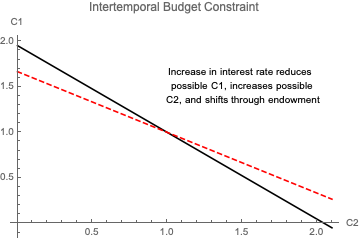
\includegraphics[scale=0.7]{ITBC3.png}\\
How should consumption respond to a change in the interest rate?
\end{figure}
\end{frame}

\begin{frame}
\frametitle[alignment=center]{Intertemporal Consumption}
\begin{itemize}
\item How should consumption respond to an increase in the interest rate?
\bigskip
\item It depends on if you were a borrower or a saver!
\bigskip
\item Idea for borrowers
\begin{itemize}
\item Interest rate increase has substitution effect: $c_1\downarrow,\ c_2\uparrow$
\item Interest rate increase has negative income effect: $c_1\downarrow,\ c_2\downarrow$
\item Sum effect is $c_1 (\downarrow)$, $c_2 (?)$
\end{itemize}
\item Idea for lenders
\begin{itemize}
\item Interest rate increase has substitution effect: $c_1\downarrow,\ c_2\uparrow$
\item Interest rate increase has positive income effect: $c_1\uparrow,\ c_2\uparrow$
\item Sum effect is $c_1 (?)$, $c_2 (\uparrow)$
\end{itemize}
\item Note that for everyone, we expect $c_2/c_1\uparrow$ (Prediction 4:  $c_2/c_1$ should increase when interest rates increase)
\item Let's see these ideas graphically
\end{itemize}
\end{frame}

\begin{frame}
\frametitle[alignment=center]{Testable Predictions-II}
\begin{figure}
\centering
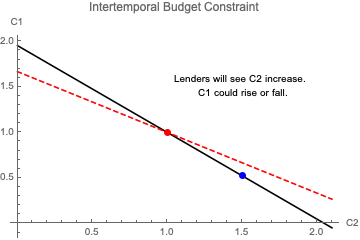
\includegraphics[scale=0.7]{ITBC4.png}\\
\end{figure}
In general probably expect both to go down
\end{frame}

\begin{frame}
\frametitle[alignment=center]{Testable Predictions-II}
\begin{figure}
\centering
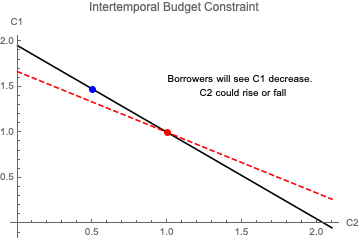
\includegraphics[scale=0.7]{ITBC5.png}\\
\end{figure}
 In general probably expect both to go up
\end{frame}

\begin{frame}
\frametitle[alignment=center]{Other predictions of the smoothing framework: labor}
\begin{itemize}
\item What are other predictions?
\bigskip
\item We know if your wage goes up forever, probably don't work \emph{much} more or less (income and substitution effects cancel or mostly cancel)
\bigskip
\item But what if your wage goes up this period?
\bigskip
\item<2-> Should see an increase in labor!  (why?
\bigskip
\item<3->  Little income effect, big substitution effect!
\bigskip
\item Let's look at evidence/tests for some of these hypotheses!
\end{itemize}
\end{frame}


\begin{frame}
\frametitle[alignment=center]{Other predictions of the smoothing framework: labor}
\begin{itemize}
\item What are other predictions?
\bigskip
\item We know if your wage goes up forever, probably don't work \emph{much} more or less (income and substitution effects cancel or mostly cancel)
\bigskip
\item But what if your wage goes up this period?
\bigskip
\item<2-> Should see an increase in labor!  (why?
\bigskip
\item<3->  Little income effect, big substitution effect!
\bigskip
\item Let's look at evidence/tests for some of these hypotheses!
\item Prediction 5:  Permanent wage changes should not affect long-run labor
\item Prediction 6:  Temporary wage changes should strongly effect short-run labor
\end{itemize}
\end{frame}

\begin{frame}
\frametitle{Prediction 1: Income Timing}
\begin{itemize}
\item The first prediction is that it doesn't matter when in our lives we get our income.  If we get it all now, we save it.  If we get it all in the future, we go into debt then pay it off when we get the income.  
\bigskip
\item Data/Experiment:  Alaskans get (or used to get) \$8000/person each year in fourth quarter
\bigskip
\item Result:  Alaskan households had smooth consumptions throughout the year: debt three quarters, save last quarter.
\bigskip
\item Data/Experiment:  Households get sometimes large or surprise tax refunds in U.S.
\bigskip
\item Result:  Households do not see large increases in consumption.
\end{itemize}
\end{frame}


\begin{frame}
\frametitle{Prediction 2: Marginal Propensity to Consume}
\begin{itemize}
\item Prediction:  a large one-time increase in income should not be spent today, but instead smoothed over many periods  
\bigskip
\item Data/Experiment:  Restitution payments to Israeli citizens from Germany ($\approx$ 1 years income).
\bigskip
\item Result:  Total expenditure increased by 20\% of amount (mostly in durable goods, which are savings)
\bigskip
\item Data/Experiment:  WWII veterans got a one-time life-insurance dividend of \$175 (4\% annual income)
\bigskip
\item Result:  Expenditure rose by 35\% of the amount, but again mostly in durable goods.
\bigskip
\item Additional fact:  a large \textbf{permanent} increase in income is met with approximately the same size increase in consumption. 
\end{itemize}
\end{frame}

\begin{frame}
\frametitle{Prediction 3: Anticipated Income Changes}
\begin{itemize}
\item Prediction:  consumption should not change when income is predicted to change
\bigskip
\item Data/Experiment:  Alaskan example (they don't): 10\% increase in household income increases consumption by 0.2\%(!)
\bigskip
\item Data/Experiment: Income tax refunds:  consumption only increases by 10\% of amount
\end{itemize}
\end{frame}

\begin{frame}
\frametitle{Prediction 4: Interest Rates}
\begin{itemize}
\item Another prediction we have is that a higher interest rate reduces current consumption \textbf{compared to} future consumption $c_2/c_1$.  
\item Also, Higher interest rates mean households should work now
\bigskip
\item Data/Experiment:  Longitudinal data on U.S. household purchases
\bigskip
\item Result:  A 1 percentage point increase in the interest rate increases $c_2/c_1$ by about 0.5 percentage points/year.
\bigskip
\item Data/Experiment:  Aggregate economy
\bigskip
\item Result:  A 1 percentage point increase in the interest rate increases $c_2/c_1$ by about 0.3 percentage points/year.
\bigskip
\item Data/Experiment:  Data on annual interest rates
\bigskip
\item Result:  A 1 percentage point increase in the interest rate increases $L_2/L_1$ by about 0.2-0.6 percentage points/year.
\end{itemize}
\end{frame}


\begin{frame}
\frametitle{Prediction 5: Permanent wages changes}
\begin{itemize}
\item When households get permanently higher wages, it's unclear what they should do, income and substitution effects offset  
\bigskip
\item Data/Experiment:  Long-run wage increases in U.S.
\bigskip
\item Result:  Little change in long-run labor
\end{itemize}
\end{frame}

\begin{frame}
\frametitle{Prediction 6: Temporary wage changes}
\begin{itemize}
\item When households get temporarily higher wages, income effects are small but substitution effects are big: work more
\item When wages will be higher in the future, move labor to the future
\bigskip
\item Data/Experiment:  Data on employee expectations about wages
\bigskip
\item Result:  An increase in expectations about $w_2/w_1$ by 1 percentage point increased $L_2/L_1$ by 1 percentage point.
\bigskip
\item Data/Experiment:  Exxon Valdez spill
\bigskip
\item Result:  A temporary increase in real wage rates by 1\% increased hours worked per week by 2\%
\end{itemize}
\end{frame}


\begin{frame}
\frametitle{Frontier of research}
\begin{itemize}
\item The important lesson for public policy is people aren't dumb animals, they intertemporally maximize to a significant degree
\bigskip
\item However, reason to think that there are some households that are ``hand-to-mouth" liquidity constrained.  No intertemporal budget constraint for them, because they can't borrow ($s$ can't be negative).
\bigskip
\item  For these guys, reason to think that lump-sum transfers will be spent mostly today
\bigskip
\item Some evidence that it's roughly 50\% of population (Mankiw et al. 1982, structural model)
\end{itemize}
\end{frame}

\begin{frame}
\frametitle{Wealthy hand to mouth}
\begin{itemize}
\bigskip
\item Weidner, Kaplan, and Violante look carefully at marginal propensity to consume 
\bigskip
\item Examine illiquid assets and liquid assets separately
\bigskip
\item Wealthy hand-to-mouth have high MPC but illiquid assets above \$1 (or \$1000)
\bigskip
\item Shockingly, 31\% of all U.S. household ``hand-to-mouth"
\bigskip
\item Even more shockingly, 61\% of them are ``wealthy" hand to mouth
\bigskip
\item Put another way:  12\% poor hand-to-mouth, 19\% rich hand-to-mouth, 69\% not hand to mouth.
\bigskip
\item \textbf{If} want to increase consumption, not clear only tagging poor is effective!
\end{itemize}
\end{frame}

\begin{frame}
\frametitle[alignment=center]{Testable Predictions-II}
\begin{figure}
\centering
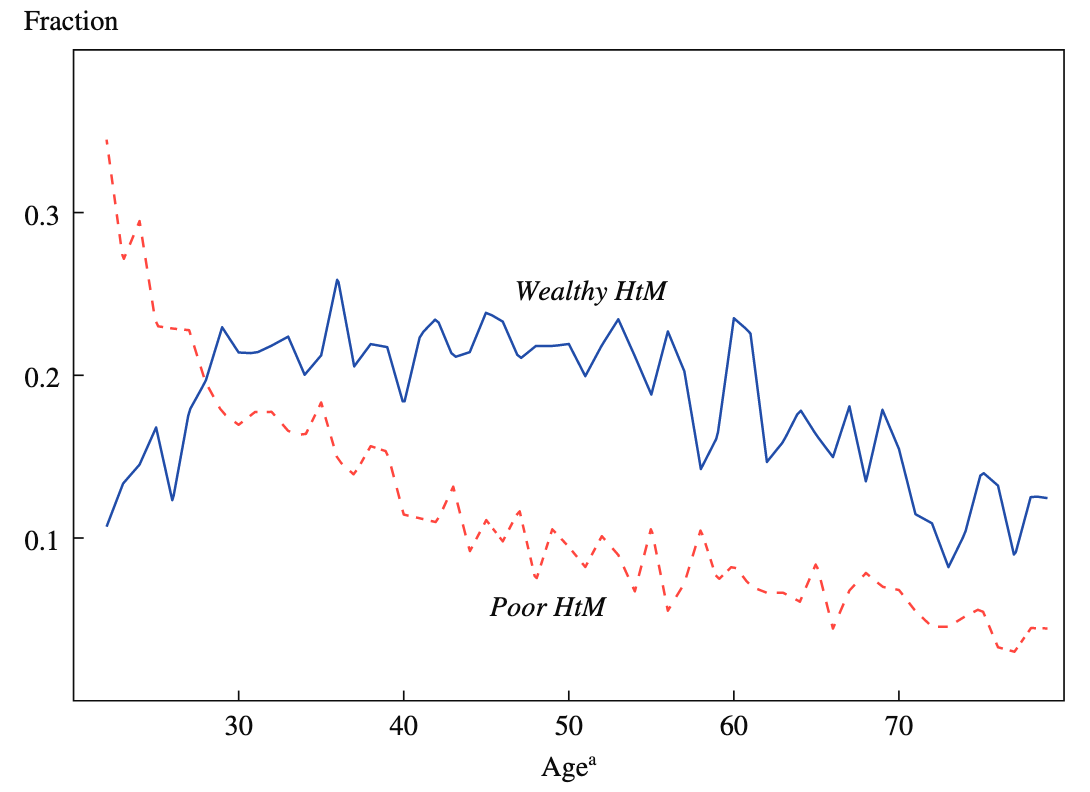
\includegraphics[scale=0.5]{HtM.png}\\
\end{figure}
\end{frame}

\begin{frame}
\frametitle[alignment=center]{Another test:  Unemployment insurance}
\begin{itemize}
\item A clear prediction of our labor and intertemporal studies regards unemployment insurance
\bigskip
\item How should people respond to the presence of unemployment insurance?
\bigskip
\item Small income effect, but big substitution effect!  If replaces 50\% of my wage gains then looks like a 50\% tax to me on the extensive margin!
\bigskip
\item Prediction:  UI benefits should strongly dissuade labor  (reduce by 37.5\%, if Frisch is 0.75 and tax is 50\% extra)
\bigskip
\item Let's look at the data
\end{itemize}
\end{frame}

\begin{frame}
\frametitle[alignment=center]{Probability of Finding Job Conditional on UI Weeks Left}
\begin{figure}
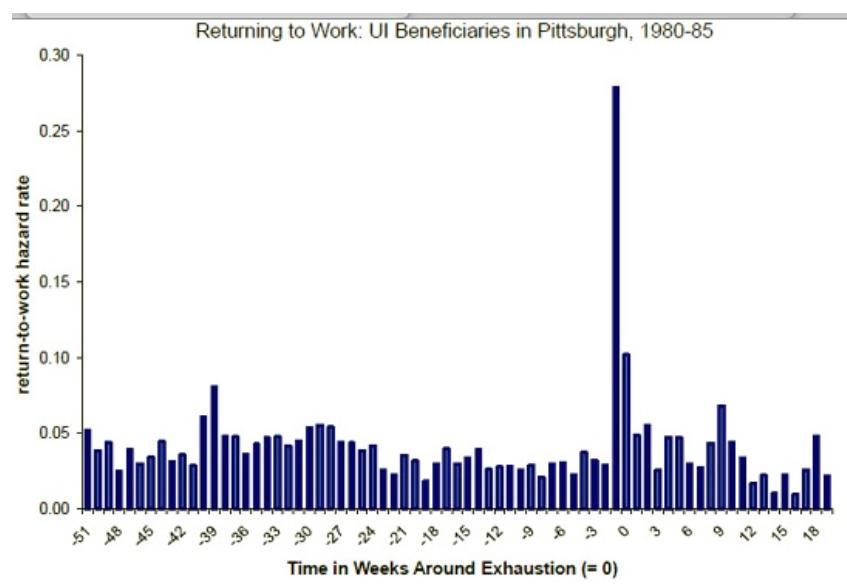
\includegraphics[scale=0.3]{UI_1.png}
\end{figure}
Jurajda and Tannery, 2003
\end{frame}

\begin{frame}
\frametitle[alignment=center]{Probability of Finding Job Conditional on UI Weeks Left}
\begin{figure}
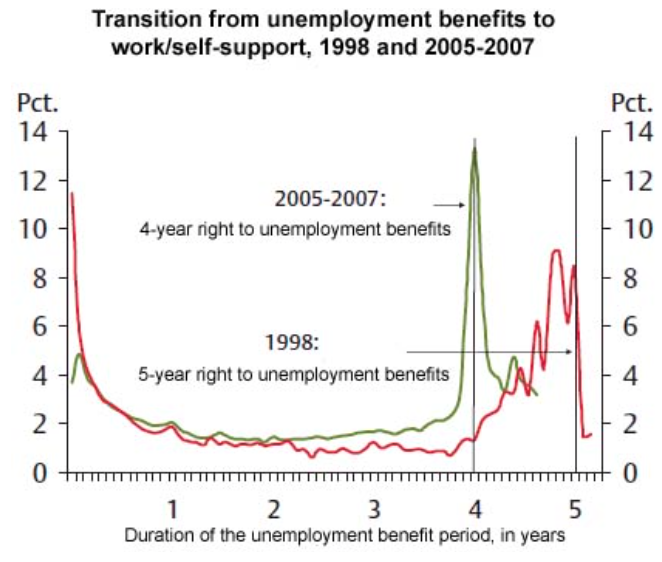
\includegraphics[scale=0.4]{UI_2.png}
\end{figure}
\end{frame}


\begin{frame}
\frametitle[alignment=center]{Probability of Finding Job Conditional on UI Weeks Left}
\begin{figure}
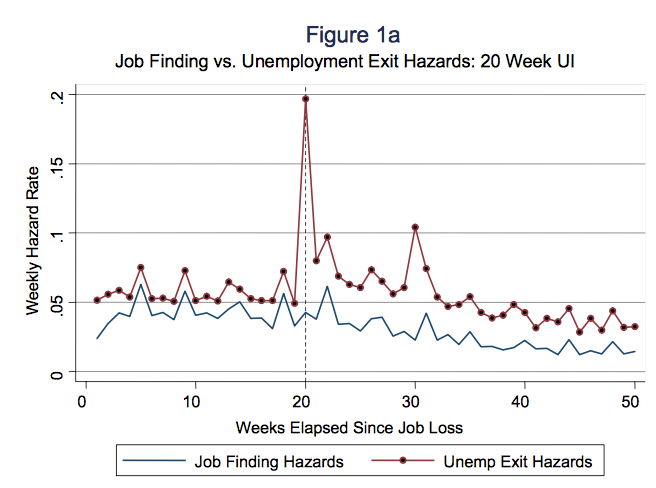
\includegraphics[scale=0.4]{UI_3.png}
\end{figure}
Card, Chetty, Weber 
\end{frame}


\begin{frame}
\frametitle[alignment=center]{Probability of Finding Job Conditional on UI Weeks Left}
\begin{figure}
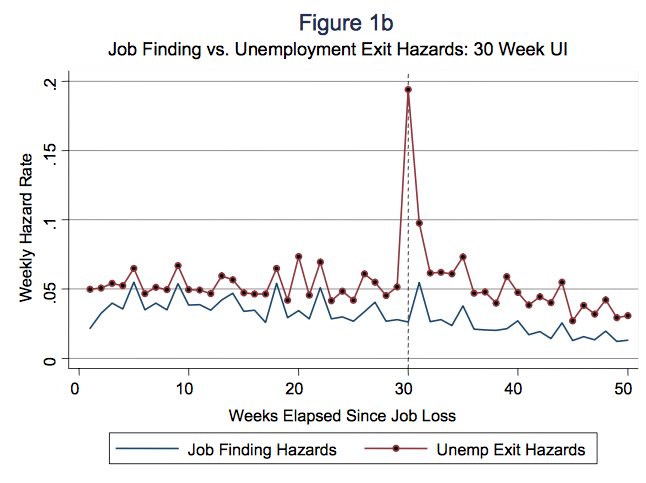
\includegraphics[scale=0.4]{UI_4.png}
\end{figure}
Card, Chetty, Weber 
\end{frame}

\begin{frame}
\frametitle[alignment=center]{Liquidity or Moral Hazard?}
\begin{itemize}
\item This isn't necessarily evidence people respond to incentives!
\bigskip
\item Could just be that people are forced to get bad jobs when they run out of money
\bigskip
\item One possible test:  benefits top out...if higher benefits mean longer search, then should see kink in duration at same place as kink in  
\end{itemize}
\end{frame}


\begin{frame}
\frametitle[alignment=center]{UI Benefits Suddenly Kink}
\begin{figure}
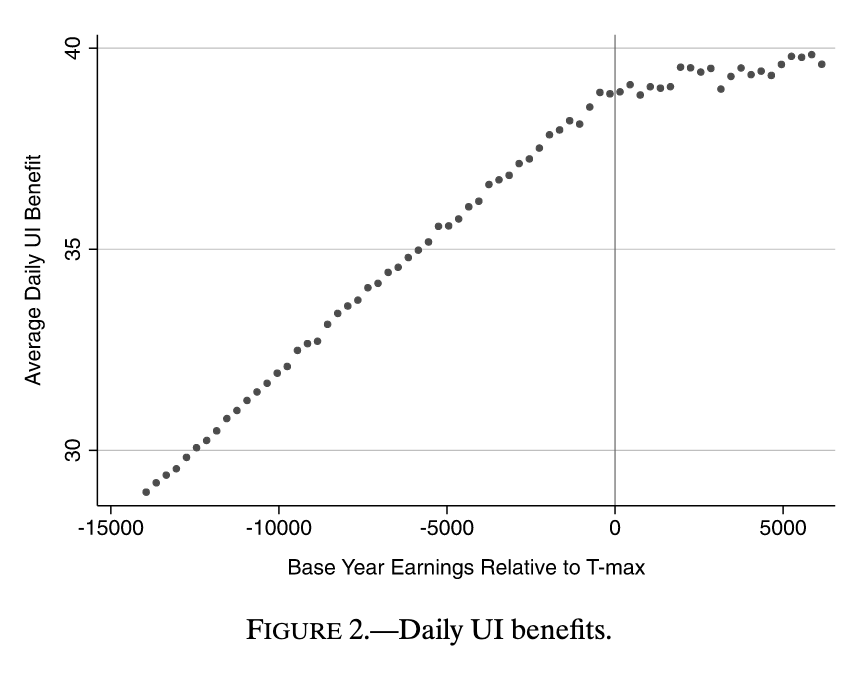
\includegraphics[scale=0.6]{CardLeePeiWeber1.png}
\end{figure}
Card, Lee, Pei, Weber  (2015)
\end{frame}

\begin{frame}
\frametitle[alignment=center]{Job Search Follows Kink!}
\begin{figure}
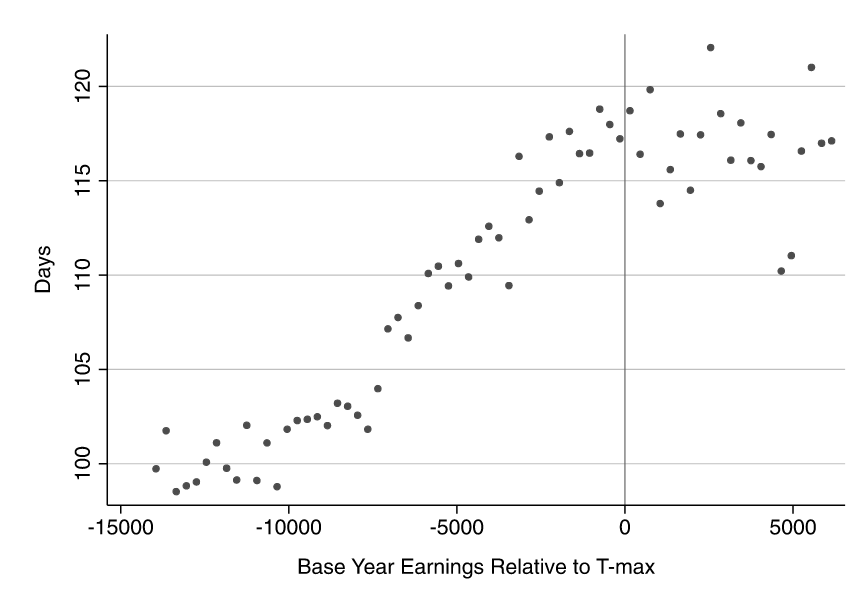
\includegraphics[scale=0.6]{CardLeePeiWeber2.png}
\end{figure}
Card, Lee, Pei, Weber  (2015)
\end{frame}

\begin{frame}
\frametitle[alignment=center]{Rejoinder}
\begin{itemize}
\item Other tests?
\bigskip
\item Chetty 2008:  do households that get severances take a long time? (if so, liquidity, not moral hazard)
\bigskip
\item Do increases in benefits affect liquidity-constrained households more (if so, liquidity, not moral hazard)
\bigskip
\item Evidence:  yes to both! Estimate:  40\% of $\frac{\Delta duration}{\Delta benefits}$ due to incentives  
\end{itemize}
\end{frame}

\begin{frame}
\frametitle[alignment=center]{Households with Mortgages React to Benefits}
\begin{figure}
\includegraphics[scale=0.6]{HHWmort.png}
\end{figure}
Chetty 2008
\end{frame}

\begin{frame}
\frametitle[alignment=center]{Households without Mortgages Don't React to Benefits}
\begin{figure}
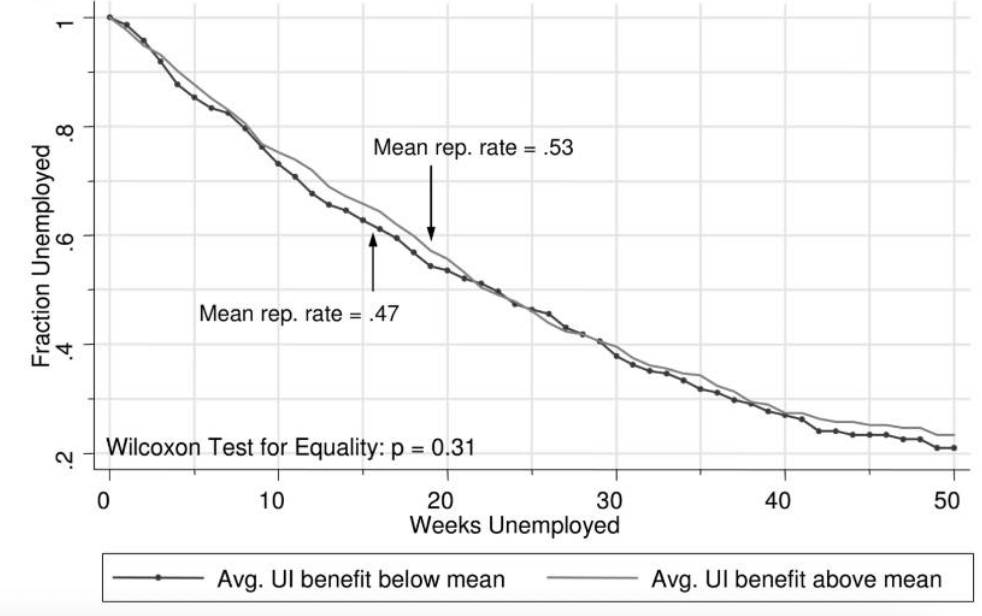
\includegraphics[scale=0.6]{HHWomort.png}
\end{figure}
Chetty 2008
\end{frame}


\begin{frame}
\frametitle[alignment=center]{Summary}
\begin{itemize}
\item The labor and consumption of households respond strongly to intertemporal incentives
\bigskip
\item Many testable predictions that come out well for theory
\bigskip
\item Unemployment insurance a particularly fruitful example
\bigskip
\item Clear that UI duration and benefits strongly effect probability of finding a job
\bigskip
\item Some of that comes from liquidity (break in intertemporal BC) but much comes from static labor incentives
\end{itemize}
\end{frame}

\end{document}